\pdfinfoomitdate=1
\pdftrailerid{}
\documentclass[12pt]{article}
\usepackage[letterpaper,margin=0.65in,headheight=16pt,headsep=18pt,footskip=25pt]{geometry}
\usepackage{tikz,amsmath,array,fancyhdr}
\usetikzlibrary{arrows.meta,patterns}
\usepackage[T1]{fontenc}
\usepackage{lmodern}
\renewcommand{\familydefault}{\sfdefault}
\pagestyle{fancy}\fancyhf{}
\fancyhead[L]{\small Week 89 / Growing shapes and totals / Grades K--5}
\fancyfoot[L]{\small Bellingham Math Circle / Week 89 / W89-S-v2}
\fancyfoot[R]{\small\thepage}
\renewcommand{\headrulewidth}{0.4pt}\renewcommand{\footrulewidth}{0pt}
\setlength{\parindent}{0pt}\setlength{\parskip}{9pt}
\newcommand{\problem}[2]{\textbf{Problem #1:} #2\par}
\newcommand{\answer}[1]{\par\vspace{#1}\par}
\newcommand{\tile}[3]{\filldraw[fill=#3,draw=black!65,line width=.35pt] (#1,#2) rectangle ++(1,1);}
\newcommand{\squarefig}[1]{\begin{tikzpicture}[x=5mm,y=5mm,baseline=(current bounding box.center)]\foreach \x in {1,...,#1}{\foreach \y in {1,...,#1}{\tile{\x}{\y}{white}}}\end{tikzpicture}}
\newcommand{\stairfig}[1]{\begin{tikzpicture}[x=5mm,y=5mm,baseline=(current bounding box.center)]\foreach \y in {1,...,#1}{\foreach \x in {1,...,\y}{\tile{\x}{#1-\y}{white}}}\end{tikzpicture}}
\newcommand{\rectfig}[1]{\begin{tikzpicture}[x=5mm,y=5mm,baseline=(current bounding box.center)]\pgfmathtruncatemacro{\w}{#1+1}\foreach \x in {1,...,\w}{\foreach \y in {1,...,#1}{\tile{\x}{\y}{white}}}\end{tikzpicture}}
\newcommand{\slips}[1]{\begin{tikzpicture}[baseline=(current bounding box.center)]\foreach \a [count=\i from 0] in {#1}{\draw (\i*1.1,0) rectangle ++(.85,.75);\node at (\i*1.1+.425,.375){\Large\a};}\end{tikzpicture}}
\newcommand{\tray}[4]{\draw[rounded corners=3pt] (#1,#2) rectangle ++(1.65,1.15);\node at (#1+.825,#2+.63){\Large #4};\node[font=\small] at (#1+.825,#2-.25){#3};}
\begin{document}

Use square tiles on the large boards or the tabletop. Build one picture at a time. Keep the old tiles in place when you grow a shape.

\begin{center}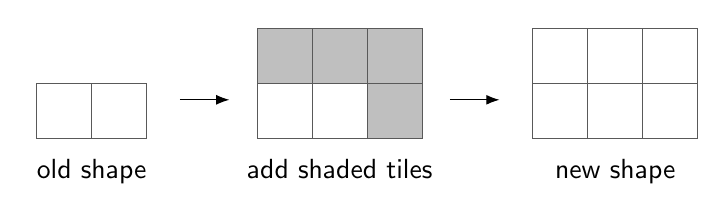
\begin{tikzpicture}[x=7mm,y=7mm]
\tile{0}{0}{white}\tile{1}{0}{white}
\node[below] at (1,-.2){old shape};
\draw[-{Latex}] (2.6,.7)--(3.5,.7);
\tile{4}{0}{white}\tile{5}{0}{white}\tile{6}{0}{black!25}
\foreach \x in {4,5,6}{\tile{\x}{1}{black!25}}
\node[below] at (5.5,-.2){add shaded tiles};
\draw[-{Latex}] (7.5,.7)--(8.4,.7);
\foreach \x in {9,10,11}{\foreach \y in {0,1}{\tile{\x}{\y}{white}}}
\node[below] at (10.5,-.2){new shape};
\end{tikzpicture}\end{center}

\problem{1}{Make each square, then grow it into the next square. What tiles must you add?}

\begin{center}\begin{tabular}{cccc}
\squarefig{1}&\squarefig{2}&\squarefig{3}&\squarefig{4}\\[8pt]
side 1&side 2&side 3&side 4
\end{tabular}\end{center}
\answer{25mm}

\problem{2}{Make a square with side 5. Take away tiles to leave a smaller square tucked into its bottom-left corner; find every possible size.}

\begin{center}\squarefig{5}\end{center}

\newpage

\problem{3}{Grow these stairs. Add one new bottom row each time, with one more tile than the row above it. Make stairs with 2, 3, 4, 5 and 6 rows.}

\begin{center}\begin{tabular}{cccc}
\stairfig{1}&\stairfig{2}&\stairfig{3}&\stairfig{4}\\[8pt]
1 row&2 rows&3 rows&4 rows
\end{tabular}\end{center}
\answer{35mm}

\problem{4}{Make two copies of the same stairs. Fit them together into a rectangle with no gaps or overlaps. Do it for stairs with 2, 3, 4, 5 and 6 rows.}

\begin{center}\stairfig{3}\hspace{20mm}\stairfig{3}\end{center}
\answer{35mm}

\newpage

\problem{5}{Grow these rectangles to 6 rows. Each rectangle has one more column than rows. What layer must you add each time?}

\begin{center}\begin{tabular}{cccc}
\rectfig{1}&\rectfig{2}&\rectfig{3}&\rectfig{4}\\[8pt]
1 row&2 rows&3 rows&4 rows
\end{tabular}\end{center}
\answer{24mm}

\problem{6}{For squares, stairs and these rectangles, how does the number of added tiles change from one growth to the next? Find a rule that works however far you grow.}

\begin{center}\renewcommand{\arraystretch}{2.2}
\begin{tabular}{l|ccccc}
added tiles&1 to 2&2 to 3&3 to 4&4 to 5&5 to 6\\\hline
squares&&&&&\\\hline
stairs&&&&&\\\hline
rectangles&&&&&
\end{tabular}\end{center}

\newpage

\problem{7}{Can the order of these inputs change the final total? Use each shown input once. Try a tray starting at 0, then a tray starting at 3.}

\begin{center}\slips{0,1,2,3,4}\end{center}
Use the supplied input cards. An input tells how many counters to add. Keep the counters already in the tray. The number in the tray is its total. You may replace counters by one card showing their total.

\begin{center}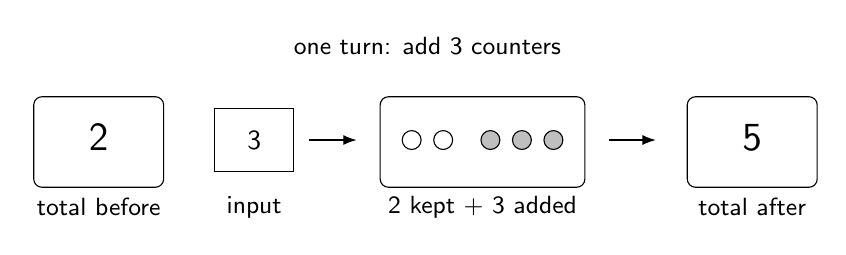
\begin{tikzpicture}[x=1cm,y=1cm]
\tray{0}{0}{total before}{2}
\node[draw,minimum width=1cm,minimum height=.8cm] at (2.8,.6){3};
\node[font=\small] at (2.8,-.25){input};
\draw[-{Latex}] (3.5,.6)--(4.1,.6);
\draw[rounded corners=3pt] (4.4,0) rectangle (7,1.15);
\foreach \x in {4.8,5.2}{\filldraw[fill=white] (\x,.6) circle (.12);}
\foreach \x in {5.8,6.2,6.6}{\filldraw[fill=black!25] (\x,.6) circle (.12);}
\node[font=\small] at (5.7,-.25){2 kept + 3 added};
\draw[-{Latex}] (7.3,.6)--(7.9,.6);
\tray{8.3}{0}{total after}{5}
\node[font=\small,align=center] at (5,1.8){one turn: add 3 counters};
\end{tikzpicture}\end{center}
\answer{20mm}

\problem{8}{Find the missing inputs. These are the totals after each turn. The tray starts at 2.}

\begin{center}\renewcommand{\arraystretch}{2}
\begin{tabular}{c|cccc}
turn&1&2&3&4\\\hline
total&5&5&9&12\\
input&\underline{\hspace{12mm}}&\underline{\hspace{12mm}}&\underline{\hspace{12mm}}&\underline{\hspace{12mm}}
\end{tabular}\end{center}

\newpage

\problem{9}{Someone hid the starting total and all four inputs. Every input was a whole number from 0 to 5. Find every possible starting total and its four inputs.}

\begin{center}\renewcommand{\arraystretch}{2}
\begin{tabular}{c|cccc}
turn&1&2&3&4\\\hline
total&4&7&7&12
\end{tabular}\end{center}
\answer{55mm}

\problem{10}{Two trays receive the same inputs: 2, 0, 3, 1. One starts at 1 and the other at 4. How far apart are their totals after each turn? What can you say for any shared input list?}

\answer{40mm}

\newpage

\problem{11}{Arrange the five inputs to make the second tray finish as large as possible. Then make it as small as possible. Start both totals at 0 each time.}

\begin{center}\slips{2,2,1,0,0}\end{center}
Each turn, add the input to the first total. Then add a copy of the \emph{new first total} to the second total. Keep both totals; nothing moves out of either tray. Use one total card in each tray and change it when needed.

\begin{center}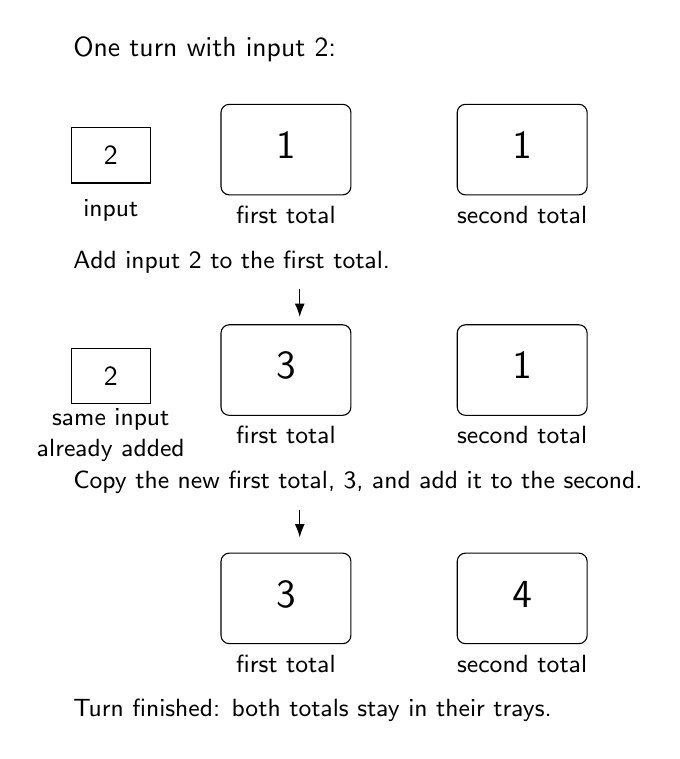
\begin{tikzpicture}[x=1cm,y=1cm]
\node[anchor=west] at (0,7.15){One turn with input 2:};
\node[draw,minimum width=1cm,minimum height=.7cm] at (.6,5.8){2};
\node[font=\small] at (.6,5.1){input};
\tray{2}{5.3}{first total}{1}\tray{5}{5.3}{second total}{1}
\node[font=\small,anchor=west] at (0,4.45){Add input 2 to the first total.};
\draw[-{Latex}] (3,4.1)--(3,3.75);
\node[draw,minimum width=1cm,minimum height=.7cm] at (.6,3){2};
\node[font=\small,align=center] at (.6,2.25){same input\\already added};
\tray{2}{2.5}{first total}{3}\tray{5}{2.5}{second total}{1}
\node[font=\small,anchor=west] at (0,1.65){Copy the new first total, 3, and add it to the second.};
\draw[-{Latex}] (3,1.3)--(3,.95);
\tray{2}{-.4}{first total}{3}\tray{5}{-.4}{second total}{4}
\node[font=\small,anchor=west] at (0,-1.25){Turn finished: both totals stay in their trays.};
\end{tikzpicture}\end{center}
\vspace{6mm}
Largest final second total: \underline{\hspace{19mm}}\quad order: \underline{\hspace{50mm}}

Smallest final second total: \underline{\hspace{19mm}}\quad order: \underline{\hspace{50mm}}

\newpage

\problem{12}{Where should the two zeros go to make the second total largest? Where should they go to make it smallest? Keep the 1 before the 3. Start both trays at 0.}

\begin{center}\slips{1,3}\hspace{12mm}\slips{0,0}\end{center}
A zero input is a whole turn: add 0 to the first total, then add a copy of that first total to the second.
\answer{55mm}

\problem{13}{Return to the inputs 2, 2, 1, 0, 0. Explain why your largest and smallest final second totals cannot be beaten. Would your ordering rule still work with any five nonnegative inputs?}

\answer{65mm}

\newpage

\problem{14}{These four pictures fit both building rules below. Use each rule to build steps 5 and 6. Do the first four pictures decide what step 5 must be?}

\begin{center}\begin{tabular}{cccc}
\squarefig{1}&\squarefig{2}&\squarefig{3}&\squarefig{4}\\[8pt]
step 1&step 2&step 3&step 4
\end{tabular}\end{center}
\vspace{3mm}
Rule A: At every step, make a square whose side equals the step number.

Rule B: Make that same square. After step 4, attach a single row of extra tiles to the right of its bottom row: 1 extra at step 5, 2 at step 6, 3 at step 7, and so on.
\answer{32mm}

\problem{15}{Invent a third building rule that matches all four pictures and gives a different step 5 from both rules above. Your rule must say what to build at every later step too.}

\answer{35mm}

\newpage

\problem{16}{Grow a solid cube from side 1 to side 2, then to side 3, then to side 4. Each time keep the old cube in one corner. How many new cubes belong to each shell?}

\begin{center}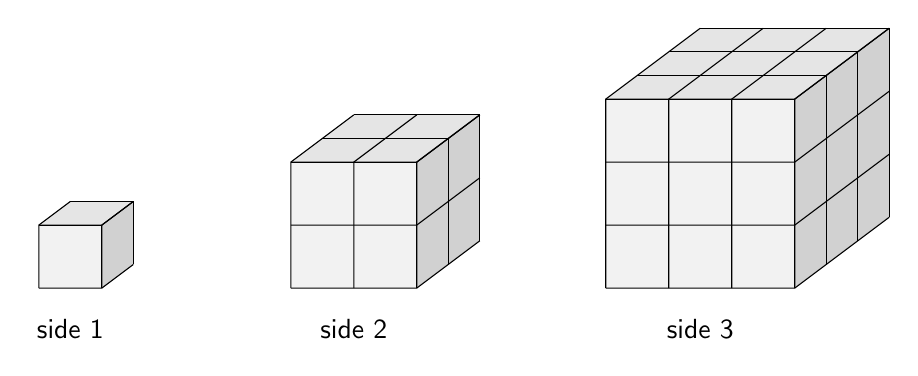
\begin{tikzpicture}[x={(8mm,0)},y={(4mm,3mm)},z={(0,8mm)}]
\foreach \a/\xx in {1/0,2/4,3/9}{
\begin{scope}[shift={(\xx,0,0)}]
\fill[black!5] (0,0,0)--(\a,0,0)--(\a,0,\a)--(0,0,\a)--cycle;
\fill[black!18] (\a,0,0)--(\a,\a,0)--(\a,\a,\a)--(\a,0,\a)--cycle;
\fill[black!10] (0,0,\a)--(\a,0,\a)--(\a,\a,\a)--(0,\a,\a)--cycle;
\foreach \k in {0,...,\a}{\draw (\k,0,0)--(\k,0,\a)--(\k,\a,\a);\draw (0,0,\k)--(\a,0,\k)--(\a,\a,\k);\draw (0,\k,\a)--(\a,\k,\a)--(\a,\k,0);}
\node at (\a/2,0,-.65){side \a};
\end{scope}}
\end{tikzpicture}\end{center}
\answer{30mm}

\problem{17}{Split a new shell into three flat rectangular slabs, with no cube used twice. Can your split work for any old side length? Use it to explain the number of cubes in the shell.}

\answer{55mm}

\newpage

\problem{18}{What changes if a third tray keeps adding copies of the second total? Start three trays at 0 and use input 1 for six turns. Find a rule for each tray's total after any number of turns.}

On each turn, update the first tray, then the second, then the third. Each tray keeps its previous total. Copy each total only after it has been updated on that turn.

\begin{center}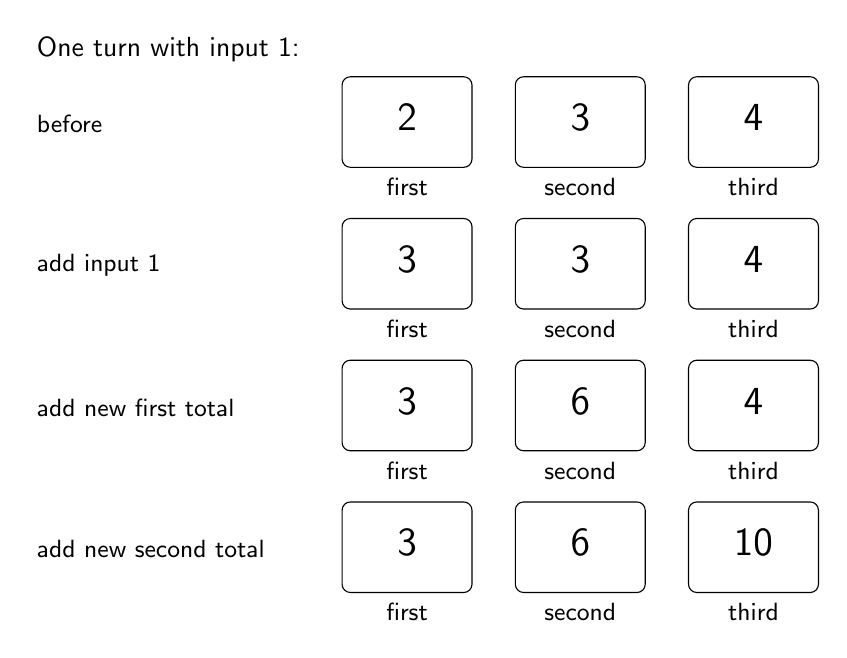
\begin{tikzpicture}[x=1cm,y=1cm]
\node[anchor=west] at (0,4.6){One turn with input 1:};
\foreach \yy/\aa/\bb/\cc/\txt in {3.1/2/3/4/before,1.3/3/3/4/add input 1,-0.5/3/6/4/add new first total,-2.3/3/6/10/add new second total}{
\node[anchor=west,font=\small] at (0,\yy+.55){\txt};
\tray{4}{\yy}{first}{\aa}\tray{6.2}{\yy}{second}{\bb}\tray{8.4}{\yy}{third}{\cc}}
\end{tikzpicture}\end{center}
\answer{15mm}
\begin{center}\renewcommand{\arraystretch}{2}
\begin{tabular}{c|ccc}
turns&first total&second total&third total\\\hline
6&&&
\end{tabular}\end{center}

\newpage

\problem{19}{Build these corner piles for steps 3, 4 and 5. Can they explain the third tray's totals when every input is 1?}

At step 1, use one cube. At step 2, stack the step-1 pile on a bottom layer of 2-row stairs. At step 3, stack the step-2 pile on a bottom layer of 3-row stairs. Continue in the same way, keeping the square corners aligned.

\begin{center}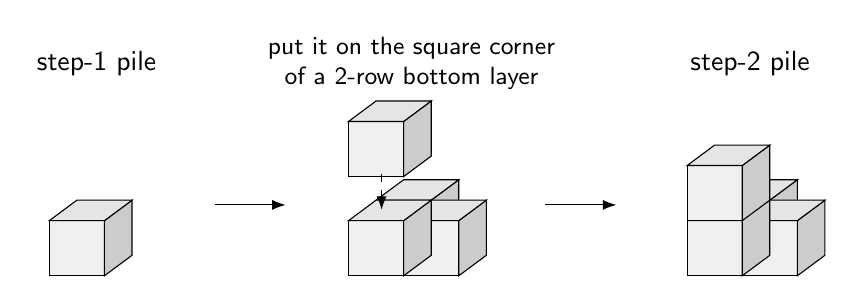
\begin{tikzpicture}[x=1cm,y=1cm]
\node at (1,3){step-1 pile};
\begin{scope}[shift={(.4,.3)},x={(7mm,0)},y={(3.5mm,2.6mm)},z={(0,7mm)}]
\filldraw[fill=black!6] (0,0,0)--(1,0,0)--(1,0,1)--(0,0,1)--cycle;
\filldraw[fill=black!20] (1,0,0)--(1,1,0)--(1,1,1)--(1,0,1)--cycle;
\filldraw[fill=black!10] (0,0,1)--(1,0,1)--(1,1,1)--(0,1,1)--cycle;
\end{scope}\draw[-{Latex}] (2.5,1.2)--(3.4,1.2);\node[align=center,font=\small] at (5,3){put it on the square corner\\of a 2-row bottom layer};\begin{scope}[shift={(4.2,.3)},x={(7mm,0)},y={(3.5mm,2.6mm)},z={(0,7mm)}]
\filldraw[fill=black!6] (0,1,0)--(1,1,0)--(1,1,1)--(0,1,1)--cycle;
\filldraw[fill=black!20] (1,1,0)--(1,2,0)--(1,2,1)--(1,1,1)--cycle;
\filldraw[fill=black!10] (0,1,1)--(1,1,1)--(1,2,1)--(0,2,1)--cycle;
\filldraw[fill=black!6] (1,0,0)--(2,0,0)--(2,0,1)--(1,0,1)--cycle;
\filldraw[fill=black!20] (2,0,0)--(2,1,0)--(2,1,1)--(2,0,1)--cycle;
\filldraw[fill=black!10] (1,0,1)--(2,0,1)--(2,1,1)--(1,1,1)--cycle;
\filldraw[fill=black!6] (0,0,0)--(1,0,0)--(1,0,1)--(0,0,1)--cycle;
\filldraw[fill=black!20] (1,0,0)--(1,1,0)--(1,1,1)--(1,0,1)--cycle;
\filldraw[fill=black!10] (0,0,1)--(1,0,1)--(1,1,1)--(0,1,1)--cycle;
\begin{scope}[shift={(0,0,1.8)}]\filldraw[fill=black!6] (0,0,0)--(1,0,0)--(1,0,1)--(0,0,1)--cycle;
\filldraw[fill=black!20] (1,0,0)--(1,1,0)--(1,1,1)--(1,0,1)--cycle;
\filldraw[fill=black!10] (0,0,1)--(1,0,1)--(1,1,1)--(0,1,1)--cycle;
\end{scope}\draw[dashed,-{Latex}] (.4,.4,1.7)--(.4,.4,1.05);\end{scope}\draw[-{Latex}] (6.7,1.2)--(7.6,1.2);\node at (9.3,3){step-2 pile};\begin{scope}[shift={(8.5,.3)},x={(7mm,0)},y={(3.5mm,2.6mm)},z={(0,7mm)}]
\filldraw[fill=black!6] (0,1,0)--(1,1,0)--(1,1,1)--(0,1,1)--cycle;
\filldraw[fill=black!20] (1,1,0)--(1,2,0)--(1,2,1)--(1,1,1)--cycle;
\filldraw[fill=black!10] (0,1,1)--(1,1,1)--(1,2,1)--(0,2,1)--cycle;
\filldraw[fill=black!6] (1,0,0)--(2,0,0)--(2,0,1)--(1,0,1)--cycle;
\filldraw[fill=black!20] (2,0,0)--(2,1,0)--(2,1,1)--(2,0,1)--cycle;
\filldraw[fill=black!10] (1,0,1)--(2,0,1)--(2,1,1)--(1,1,1)--cycle;
\filldraw[fill=black!6] (0,0,0)--(1,0,0)--(1,0,2)--(0,0,2)--cycle;
\filldraw[fill=black!20] (1,0,0)--(1,1,0)--(1,1,2)--(1,0,2)--cycle;
\filldraw[fill=black!10] (0,0,2)--(1,0,2)--(1,1,2)--(0,1,2)--cycle;
\draw (0,0,1)--(1,0,1)--(1,1,1);\end{scope}
\end{tikzpicture}\end{center}
\answer{20mm}

\problem{20}{How many cubes would a step-10 corner pile need? Find a way to get the total without building it or listing all ten running totals.}

\answer{40mm}

\end{document}
